% Drawing 43/04-14 -- folder 43, batch 04, archive page 67 (PDF page 68).
% Transcription: les croquis du bas de la page. En haut à gauche, un segment épaissi d'où partent des flèches vers $K(x)$, $K(x')$, $K(y)$, $K(y')$ ; en haut au centre, un segment gradué surmonté d'arcs ; au milieu, un graphe de cinq points reliés par des flèches marquées $d$, $d'_s$, $d'$, l'un des points étant $\Theta$ entouré ; à droite, un second graphe : un éventail de flèches portant les poids $1$, $2$, $3$ et des $d$ ; à gauche, deux petits segments légendés « $d$ gauche » et « gauche $d$ » ; en bas, un segment gradué sous cinq $\Theta$, un autre segment gradué, et un dernier croquis de trois points légendé « gauche $\Theta$ ».
% Kind: plate: segments, graduated segments and two graphs of arrows. Method 2 (schematic redraw from the facsimile). Status: partial.
% Notes: Ink, schematic. (1) A heavy segment with three ticks and six thin arrows between it and the labels K(x), K(x'), K(y'), K(y). (2) A graduated segment (six ticks) with four arcs over its intervals. (3) Five points: three long arrows to the right, and three short heavy arrows labelled d, d'_s, d'; the fourth point is the ringed Theta. (4) The second graph is reduced to its source point, twelve arrows fanning to the right and the weights 1, 2, 3 and letters d placed about as on the page. (5) Two small segments with three ticks each, their right half heavy, with the words « d gauche » and « gauche d » (the word is an uncertain reading of the transcription). (6) A graduated segment with seven ticks, one interval heavy, under five Theta. (7) A segment with eight ticks. (8) Three points joined by two strokes, labelled « gauche » and Theta. Left out: the words and formulas written among the sketches (H(x, K(p) -> 1, Hom(K, D(A)) and the others). Still differs: figure (4) is only indicated: on the page it is a dense bundle of about fifteen arrows between some eight points, whose incidences cannot be read reliably on the render; the weights are placed near where they stand, not attached to definite arrows. Redrawn 2026-11-12 (issue 128): to check again.
% Coordinates: 1 unit = 2 mm = 1/100 of the crop width, y downwards as on the crop (bbox in page fractions: [0.18, 0.575, 0.96, 0.875]).
% Redrawn by Claude (claude-fable-5-2), issue #128, 2026-11-12; not checked by a human; not compiled (no TeX in the session).
% Rights: reproduces part of the work -- behind RENDER_TRANSCRIPTS, never published by itself.
\documentclass[tikz,border=3pt]{standalone}
\usepackage{amsmath,amssymb}
\usetikzlibrary{patterns,arrows.meta}
\tikzset{pencil/.style={black!45}, struck/.style={black!35}, mpt/.style={circle,draw,inner sep=1.3pt}, pt/.style={circle,fill,inner sep=0.9pt}, opt/.style={circle,draw,fill=white,inner sep=1.1pt}, Rd/.style={red!75!black}, Gn/.style={green!45!black}, Br/.style={brown!70!black}}
\begin{document}
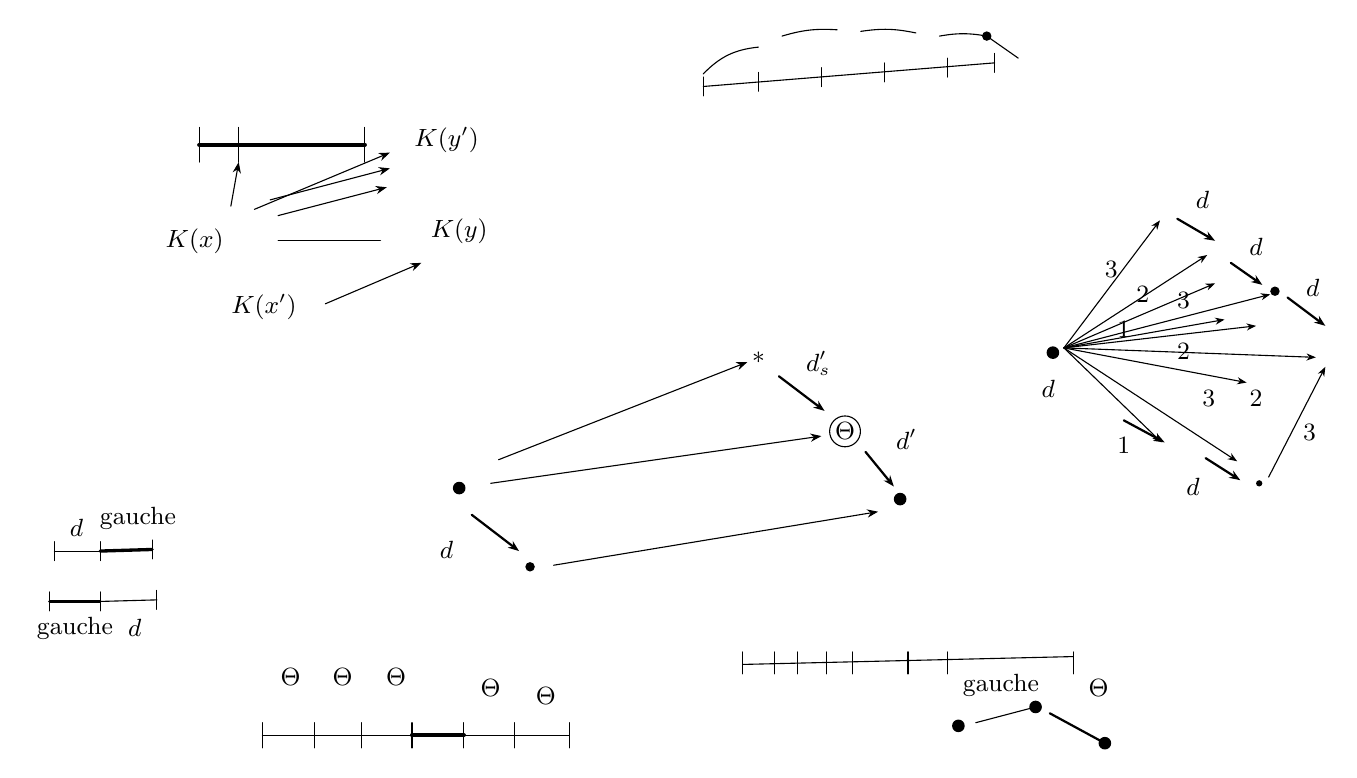
\begin{tikzpicture}[x=2mm,y=-2mm,line cap=round,line join=round,font=\small]
% (1)
\draw[line width=1.6pt] (15.5,10.5) -- (26,10.5);
\draw (15.5,9.4) -- (15.5,11.6);
\draw (18,9.4) -- (18,11.6);
\draw (26,9.4) -- (26,11.6);
\draw[-{Stealth[length=1.4mm]}] (17.5,14.4) -- (18,11.6);
\draw[-{Stealth[length=1.4mm]}] (19,14.6) -- (27.6,11);
\draw[-{Stealth[length=1.4mm]}] (20,14) -- (27.6,12);
\draw[-{Stealth[length=1.4mm]}] (20.5,15) -- (27.4,13.2);
\draw (20.5,16.6) -- (27,16.6);
\draw[-{Stealth[length=1.4mm]}] (23.5,20.6) -- (29.6,18);
\node at (15.2,16.6) {$K(x)$};
\node at (19.6,20.8) {$K(x')$};
\node at (31.2,10.2) {$K(y')$};
\node at (32,16) {$K(y)$};
% (2)
\draw (47.5,6.8) -- (66,5.3);
\foreach \x/\y in {47.5/6.8, 51/6.5, 55/6.2, 59/5.9, 63/5.6, 66/5.3} {
\draw (\x,\y-0.6) -- (\x,\y+0.6);
}
\draw (47.5,6) to[bend left=20] (51,4.3);
\draw (52.5,3.6) to[bend left=10] (56,3.2);
\draw (57.5,3.3) to[bend left=10] (61,3.4);
\draw (62.5,3.6) to[bend left=10] (65.5,3.6);
\draw (65.5,3.6) -- (67.5,5);
\fill (65.5,3.6) circle [radius=0.3];
% (3)
\coordinate (p1) at (32,32.3);
\coordinate (p2) at (36.5,37.3);
\coordinate (p3) at (51,24);
\coordinate (p4) at (56.5,28.7);
\coordinate (p5) at (60,33);
\fill (p1) circle [radius=0.4];
\fill (p2) circle [radius=0.3];
\node at (p3) {$*$};
\node[mpt,inner sep=0.6pt] at (p4) {$\Theta$};
\fill (p5) circle [radius=0.4];
\draw[-{Stealth[length=1.4mm]}] (34.5,30.5) -- (50.3,24.3);
\draw[-{Stealth[length=1.4mm]}] (34,32) -- (55,29);
\draw[-{Stealth[length=1.4mm]}] (38,37.2) -- (58.6,33.8);
\draw[thick,-{Stealth[length=1.4mm]}] (32.8,34) -- (35.8,36.3);
\draw[thick,-{Stealth[length=1.4mm]}] (52.3,25.2) -- (55.2,27.4);
\draw[thick,-{Stealth[length=1.4mm]}] (57.8,30) -- (59.6,32.2);
\node at (31.2,36.2) {$d$};
\node at (54.8,24.4) {$d'_s$};
\node at (60.4,29.2) {$d'$};
% (4)
\fill (69.7,23.7) circle [radius=0.4];
\foreach \a/\b in {76.5/15.3, 79.5/17.5, 80/19.3, 83.5/20, 80.6/21.6, 82.6/22, 86.4/24, 82/25.6, 76.6/29.4, 81.4/30.6} {
\draw[-{Stealth[length=1.2mm]}] (70.4,23.4) -- (\a,\b);
}
\draw[thick,-{Stealth[length=1.4mm]}] (77.6,15.2) -- (80,16.6);
\draw[thick,-{Stealth[length=1.4mm]}] (81,18) -- (83,19.4);
\draw[thick,-{Stealth[length=1.4mm]}] (84.6,20.2) -- (87,22);
\draw[thick,-{Stealth[length=1.4mm]}] (74.2,28) -- (76.8,29.4);
\draw[thick,-{Stealth[length=1.4mm]}] (79.4,30.4) -- (81.6,31.8);
\draw[-{Stealth[length=1.2mm]}] (83.4,31.6) -- (87,24.6);
\fill (83.8,19.8) circle [radius=0.3];
\fill (82.8,32) circle [radius=0.2];
\node at (73.4,18.4) {$3$};
\node at (75.4,20) {$2$};
\node at (78,20.4) {$3$};
\node at (74.2,22.2) {$1$};
\node at (78,23.6) {$2$};
\node at (79.6,26.6) {$3$};
\node at (82.6,26.6) {$2$};
\node at (86,28.8) {$3$};
\node at (74.2,29.6) {$1$};
\node at (79.2,14) {$d$};
\node at (82.6,17) {$d$};
\node at (86.2,19.6) {$d$};
\node at (69.4,26) {$d$};
\node at (78.6,32.2) {$d$};
% (5)
\draw (6.3,36.3) -- (9.2,36.3);
\draw[very thick] (9.2,36.3) -- (12.5,36.2);
\draw (6.3,35.7) -- (6.3,36.9);
\draw (9.2,35.7) -- (9.2,36.9);
\draw (12.5,35.6) -- (12.5,36.8);
\node at (7.7,34.8) {$d$};
\node at (11.6,34.2) {gauche};
\draw[very thick] (6,39.5) -- (9.2,39.5);
\draw (9.2,39.5) -- (12.8,39.4);
\draw (6,38.9) -- (6,40.1);
\draw (9.2,38.9) -- (9.2,40.1);
\draw (12.8,38.8) -- (12.8,40);
\node at (7.6,41.2) {gauche};
\node at (11.4,41.2) {$d$};
% (6)
\draw (19.5,48) -- (39,48);
\draw[line width=1.4pt] (29,48) -- (32.3,48);
\foreach \x in {19.5,22.8,25.8,29,32.3,35.5,39} {
\draw (\x,47.2) -- (\x,48.8);
}
\foreach \x/\y in {21.3/44.3, 24.6/44.3, 28/44.3, 34/45, 37.5/45.5} {
\node at (\x,\y) {$\Theta$};
}
% (7)
\draw (50,43.5) -- (71,43);
\foreach \x in {50,52,53.5,55.3,57,60.5,63,71} {
\draw (\x,42.7) -- (\x,44.1);
}
% (8)
\fill (63.7,47.4) circle [radius=0.4];
\fill (68.6,46.2) circle [radius=0.4];
\fill (73,48.5) circle [radius=0.4];
\draw (64.8,47.2) -- (68.6,46.2);
\draw[thick] (69.5,46.6) -- (73,48.5);
\node at (66.4,44.8) {gauche};
\node at (72.6,45) {$\Theta$};
\end{tikzpicture}
\end{document}
